%
% Capítulo 4 - Recursos/Herramientas necesarias
%
\chapter[Herramientas]{
	Herramientas
	\label{cap:herramientas}
}

Las distintas fases de trabajo del proyecto están apoyadas por un uso de software específico para su desarrollo.

Normalmente los proyectos software están desarrollados por equipos de trabajo de diversas magnitudes. Es esencial el uso de herramientas específicas que ayuden a automatizar tareas, ayudando a que el resto del equipo esté al tanto de las modificaciones realizadas.

\begin{center}{
	\fboxsep 10px
	\fcolorbox{white}{gray}{\parbox{0.95\textwidth}{
		Herramientas: RoR, latex, git, photoshop, textmate, aplicaciones web colaborativas, basecamp, pivotaltracker, jQuery, heroku
}}}\end{center}

% ----------------------------------
% Sec Ruby On Rails como framework Ruby
% ----------------------------------
\section{Ruby On Rails como framework Ruby} % (fold)
  \label{sec:ruby_on_rails_como_framework_ruby}
  
  {\it Ruby on Rails}, de ahora en adelante RoR, es una estructura de soporte para la programación web desarrollada en el lenguje Ruby por David Heinemeier Hansson, como resultado del desarrollo de {\it Basecamp} (un software para la gestión de proyectos vía web, basado en un interfaz sencillo, claro, fácil de usar, sin complicaciones). La primera versión del {\it framework} \footnote{Un {\bf framework} es una estructura conceptual y tecnológica de soporte definida, normalmente con artefactos o módulos de software concretos, con base en la cual otro proyecto de software puede ser organizado y desarrollado. Típicamente, puede incluir soporte de programas, bibliotecas y un lenguaje interpretado entre otros programas para ayudar a desarrollar y unir los diferentes componentes de un proyecto. Representa una arquitectura de software que modela las relaciones generales de las entidades del dominio. Provee una estructura y una metodología de trabajo la cual extiende o utiliza las aplicaciones del dominio.} salió a la luz pública en julio de 2004, así que RoR es muy reciente, y de ahí las reticencias que crea y la necesidad de analizar y hacer comparaciones sobre su utilidad respecto a otros soportes más consolidados.
  
  Para entender qué es RoR primero tenemos que conocer un poco en qué se apoya. RoR está programado en Ruby (ver referencias en sección \ref{sub:tec_ruby}). Los dos principios fundamentales sobre los cuáles se apoya RoR son, en primer lugar, «No te repitas» y, en segundo lugar, «Convenciones antes que configuración».
  
  % ----------------------------------
  % Sub No te repitas
  % ----------------------------------
  \subsection{No te repitas} % (fold)
    \label{sub:ror_no_te_repitas}
    
    DRY ({\it «Don't repeat yourself»}) significa que las definiciones sólo deben hacerse una vez. Como RoR es una estructura, los componentes están integrados de manera que ciertos «puentes» entre ellos no necesiten hacerse manualmente. Por ejemplo, si se tiene un formulario en la aplicación, con sólo una línea de código se puede llamar todas las veces que se quiera y donde quiera. 
    
    Otro ejemplo podría ser: en cada  tabla de la base de datos de la aplicación puedes manipular los registros de dicha tabla como si fueran atributos, sin necesidad de declarar nada, todo gracias al {\it Active Record}, uno de los patrones más llamativos de RoR.
    
    A veces, el lema «no te repitas» se expresa en otras palabras como «menos software». Menos software, menos código, significa dos cosas importantes: una es que el desarrollo se hace en menos tiempo y otra es que a menos código menos errores.
  % subsection no_te_repitas (end)
  
  % ----------------------------------
  % Sub Convenciones antes que configuración
  % ----------------------------------
  \subsection{Convenciones antes que configuración} % (fold)
    \label{sub:ror_convenciones_antes_que_configuracion}
    
    Convenciones antes que configuración significa que el programador sólo tiene que definir la configuración de aquello que no sea convencional. En muchas ocasiones definimos las cosas de la misma manera, hacemos las mismas configuraciones, con lo cual se tiende a repetir ciertos pasos una y otra vez. Estableciendo una serie de convecciones se logra ahorrar mucho tiempo porque el propio {\it framework}, por defecto, genera ciertos elementos. Por ejemplo, si se tiene en la aplicación una clase que se llama «Nadador» (nombre en singular), entonces gracias a las convenciones sabemos que en la base de datos existe una tabla que se llama «Nadadores» (nombre en plural), y así nos ahorramos escribir un montó de código a la hora de desarrollar la aplicación.
    
    Las convenciones existentes en Rails han sido definidas por el grupo de desarrolladores con la intención de facilitar el desarrollo, pero eso no implica que dichas convenciones no se puedan redefinir y cada cual configurarlas de otra manera y a su medida.
  % subsection convenciones_antes_que_configuración (end)

  % ----------------------------------
  % Sub Patrones de diseño
  % ----------------------------------
  \subsection{Patrones de diseño} % (fold)
    \label{sub:ror_patrones_de_diseno}
    
    Como se ha mencionado, {\it Ruby on Rails} es un {\it framework} para Ruby que implementa los patrones de diseño {\it Active Record} y Modelo-Vista-Controlador.
    
    % ----------------------------------
    % SubSub Active Record
    % ----------------------------------
    \subsubsection{Active Record} % (fold)
    \label{ssub:ror_active_record}
      
      {\it Active Record} es el patrón empleado por RoR para el Modelo, y soluciona el problema que surge cuando desde una programación orientada a objetos se quiere acceder a los datos de bases de datos relacionales. Con {\it Active Record}, el mapeo objeto-relacional se basa en unas pocas reglas muy sencillas: una tabla es una clase, una columna es un atributo, y una fila (tupla) es una instancia. Las relaciones entre tablas también siguen unas convenciones predefinidas: «tiene un» es una clave ajena, «tiene muchos» es una clave en otra tabla, «pertenece a» es una clave ajena y «muchos a muchos» es una tabla intermedia.
      
      El patrón {\it Active Record} permite salvar la distancia que existe entre el paradigma de la Programación Orientada a Objetos, que trata con objetos y asociaciones (paradigma más «natural»), y el modelo relacional, que trata con relaciones y conjuntos (modelo más matemático) cuando se trata de hacer persistentes los objetos del modelo de negocio.
    % subsubsection active_record (end)
    
    % ----------------------------------
    % SubSub Modelo-Vista-Controlador
    % ----------------------------------
    \subsubsection{Modelo-Vista-Controlador} % (fold)
    \label{ssub:modelo_vista_controlador}
    
    Este patrón soluciona el problema que surge cuando las vistas están acopladas a los modelos. Para desacoplarse se crea un tercer nivel que actúa como intermediación entre la Vista y el Modelo: el Controlador. El patrón MVC se basa en el principio general de desacoplar los objetos de modo que los cambios en un objeto afecten a otros pero sin necesidad de que el objeto que cambia conozco detalles de los otros.
    
    En RoR el modelo consiste en una serie de clases que representan las tablas de las bases de datos relacionales, siendo estas clases gestionadas por {\it Active Record}. La Vista es la visualización de los datos que se manejan desde las clases de los {\it Controller}. Los ficheros de la Vista tienen una extensión {\i rhtml} (puede modificarse), y contienen código Ruby embebido en HTML.
    
    Para la construcción de estos tres niveles (Modelo, Vista y Controlador), RoR ofrece un andamiaje: es lo que se llama «scaffolding». {\it Scaffolding} consiste en la construcción automática de todo el código del Modelo y de las Vistas que se necesitan para realizar las operaciones más frecuentes, como puede ser crear nuevos nadadores, ver los nadadores ya existentes, modificarlos o borrarlos, etc. Los responsables de la generación de este código son los «Scaffold Generators», generadores automáticos de código que facilitan la creación de requisitos «CRUD» (Create, Read, Update y Delete) basados en formularios web y con operaciones necesarios para el manejo de registros.
    
    % subsubsection modelo_vista_controlador (end)
  % subsection patrones_de_diseño (end)
  
  % ----------------------------------
  % Sub Servicios RESTful
  % ----------------------------------
  \subsection{Servicios RESTful} % (fold)
    \label{sub:servicios_restful}
    
    REST define un set de principios arquitectónicos por los cuales se diseñan servicios web haciendo foco en los recursos del sistema, incluyendo cómo se accede al estado de dichos recursos y cómo se transfieren por HTTP hacia clientes escritos en diversos lenguajes. REST emergió en los últimos años como el modelo predominante para el diseño de servicios. De hecho, REST logró un impacto tan grande en la web que prácticamente logró desplazar a SOAP \footnote{{\bf SOAP} (siglas de {\it Simple Object Access Protocol}) es un protocolo estándar que define cómo dos objetos en diferentes procesos pueden comunicarse por medio de intercambio de datos XML} y las interfaces basadas en WSDL \footnote {{\bf WSDL} (siglas de {\it Web Services Description Language}), un formato XML que se utiliza para describir servicios Web } por tener un estilo bastante más simple de usar.

    REST no tuvo mucha atención cuando Roy Fielding lo presentó por primera vez en el año 2000 en la Universidad de California, durante la charla academica «Estilos de Arquitectura y el Diseño de Arquitecturas de Software basadas en Redes», la cual analizaba un conjunto de principios arquitectónicos de software para usar a la Web como una plataforma de Procesamiento Distribuido.
  
    % ----------------------------------
    % SubSub Principios de REST
    % ----------------------------------
    \subsubsection{Principios de REST} % (fold)
    \label{ssub:ror_principios_de_rest}
      
      Una implementación concreta de un servicio web REST sigue cuatro principios de diseño fundamentales:
      
      \begin{enumerate}
        \item Utiliza los métodos HTTP de manera explícita
        \item No mantiene estado
        \item Expone URIs con forma de directorios
        \item Transfiere XML, JavaScript Object Notation (JSON), o ambos
      \end{enumerate}

      A continuación vamos a ver en detalle estos cuatro principios, y explicaremos porqué son importantes a la hora de diseñar un servicio web REST.
      
      \paragraph{Utiliza los métodos HTTP de manera explícita.} % (fold)
      \label{par:utiliza_los_metodos_http_de_manera_explicita}
        Una de las características claves de los servicios web REST es el uso explícito de los métodos HTTP, siguiendo el protocolo definido por RFC 2616. Por ejemplo, HTTP GET se define como un método productor de datos, cuyo uso está pensado para que las aplicaciones cliente obtengan recursos, busquen datos de un servidor web, o ejecuten una consulta esperando que el servidor web la realice y devuelva un conjunto de recursos.

        REST hace que los desarrolladores usen los métodos HTTP explícitamente de manera que resulte consistente con la definición del protocolo. Este principio de diseño básico establece una asociación uno-a-uno entre las operaciones de crear, leer, actualizar y borrar y los métodos HTTP. De acuerdo a esta asociación:

        \begin{itemize}
          \item Se usa POST para crear un recurso en el servidor
          \item Se usa GET para obtener un recurso
          \item Se usa PUT para cambiar el estado de un recurso o actualizarlo
          \item Se usa DELETE para eliminar un recurso 
        \end{itemize}
      % paragraph utiliza_los_métodos_http_de_manera_explícita (end)
  
      \paragraph{No mantiene estado.} % (fold)
      \label{par:no_mantiene_estado}
        Los servicios web REST necesitan escalar para poder satisfacer una demanda en constante crecimiento. Se usan clusters de servidores con balanceadores de carga y alta disponibilidad, {\it proxies}, y {\it gateways} de manera de conformar una topología serviciable, que permita transferir peticiones de un equipo a otro para disminuir el tiempo total de respuesta de una invocación al servicio web. El uso de servidores intermedios para mejorar la escalabilidad hace necesario que los clientes de servicios web REST envíen peticiones completas e independientes; es decir, se deben enviar peticiones que incluyan todos los datos necesarios para cumplir el pedido, de manera que los componentes en los servidores intermedios puedan redireccionar y gestionar la carga sin mantener el estado localmente entre las peticiones.

        Una petición completa e independiente hace que el servidor no tenga que recuperar ninguna información de contexto o estado al procesar la petición. Una aplicación o cliente de servicio web REST debe incluir dentro del encabezado y del cuerpo HTTP de la petición todos los parámetros, contexto y datos que necesita el servidor para generar la respuesta. De esta manera, el no mantener estado mejora el rendimiento de los servicios web y simplifica el diseño e implementación de los componentes del servidor, ya que la ausencia de estado en el servidor elimina la necesidad de sincronizar los datos de la sesión con una aplicación externa.
      % paragraph no_mantiene_estado (end)
      
      \paragraph{Expone URIs con forma de directorios.} % (fold)
      \label{par:expone_uris_con_forma_de_directorios}
      
      Desde el punto de vista del cliente de la aplicación que accede a un recurso, la URI determina qué tan intuitivo va a ser el web service REST, y si el servicio va a ser utilizado tal como fue pensado al momento de diseñarlo. La tercera característica de los servicios web REST es justamente sobre las URIs.

      Las URI de los servicios web REST deben ser intuitivas, hasta el punto de que sea facil adivinarlas. Pensemos en las URI como una interfaz auto-documentada que necesita de muy poca o ninguna explicación o referencia para que un desarrollador pueda comprender a lo que apunta, y a los recursos derivados relacionados.

      Una forma de lograr este nivel de usabilidad es definir URIs con una estructura al estilo de los directorios. Este tipo de URIs es jerárquica, con una única ruta raíz, y va abriendo ramas a través de las subrutas para exponer las áreas principales del servicio. De acuerdo a esta definición, una URI no es sólamente una cadena de caracteres delimitada por barras, sino más bien un árbol con subordinados y padres organizados como nodos.
      
      % paragraph expone_uris_con_forma_de_directorios_ (end)
      
      \paragraph{REST transfiere XML, JSON, o ambos.} % (fold)
      \label{par:rest_transfiere_xml_json_o_ambos}
        La representación de un recurso en general refleja el estado actual del mismo y sus atributos al momento en que el cliente de la aplicación realiza la petición. La representación del recurso son simples «fotos» en el tiempo. Esto podría ser una representación de un registro de la base de datos que consiste en la asociación entre columnas y tags XML, donde los valores de los elementos en el XML contienen los valores de las filas. O, si el sistema tiene un modelo de datos, la representación de un recurso es una fotografía de los atributos de una de las cosas en el modelo de datos del sistema. 

        La última restricción al momento de diseñar un servicio web REST tiene que ver con el formato de los datos que la aplicación y el servicio intercambian en las peticiones/respuestas. Acá es donde realmente vale la pena mantener las cosas simples, legibles por humanos, y conectadas.

        Los objetos del modelo de datos generalmente se relacionan de alguna manera, y las relaciones entre los objetos del modelo de datos (los recursos) deben reflejarse en la forma en la que se representan al momento de transferir los datos al cliente.
      
      % paragraph rest_transfiere_xml_json_o_ambos_ (end)
      
    % subsubsection principios_de_rest (end)
  
  % subsection servicios_restful (end)

% section ruby_on_rails_como_framework_ruby (end)

% ----------------------------------
% Sec jQuery como framework Javascript
% ----------------------------------
\section{jQuery como framework Javascript} % (fold)
  \label{sec:jquery_como_framework_javascript}

  jQuery es un framework de JavaScript, creada inicialmente por John Resig, que permite simplificar la manera de interactuar con los documentos HTML, manipular el árbol DOM, manejar eventos, desarrollar animaciones y agregar interacción con la técnica AJAX a páginas web.
  
  jQuery es software libre y de código abierto, posee un doble licenciamiento bajo la Licencia MIT y la Licencia Pública General de GNU v2, permitiendo su uso en proyectos libres y privativos. Al igual que otras bibliotecas, ofrece una serie de funcionalidades basadas en JavaScript que de otra manera requerirían de mucho más código, es decir, con las funciones propias de esta biblioteca se logran grandes resultados en menos tiempo y espacio.
  
  Entre las ventajas de uso se encuentran:
  
    \begin{itemize}
      \item {\bf Buena aceptación} por parte de los desarrolladores.
      \item {\bf Compatibilidad}. Cuando un desarrollador tiene que utilizar Javascript, generalmente tiene que preocuparse por hacer scripts compatibles con varios navegadores y para ello tiene que incorporar mucho código que lo único que hace es detectar el navegador del usuario, para hacer una u otra cosa dependiendo de si es Internet Explorer, Firefox, Opera, etc. jQuery es donde más nos puede ayudar, puesto que implementa una serie de clases (de programación orientada a objetos) que nos permiten programar sin preocuparnos del navegador con el que nos está visitando el usuario, ya que funcionan de exacta forma en todas las plataformas más habituales.
      \item {\bf Licencia gratuita}. El framework tiene licencia para uso en cualquier tipo de plataforma, personal o comercial.
      \item {\bf Liviano}. El archivo del framework ocupa unos 56 KB (19KB en caso de enviarse de manera comprimida), lo que es bastante razonable y no retrasará mucho la carga de las páginas que intervienen en el proyecto. El servidor lo enviará al cliente la primera vez que visite una página del sitio. En siguientes páginas el cliente ya tendrá el archivo del framework, por lo que no necesitará transferirlo y lo tomará de la caché. Con ello, la carga de la página sólo se verá afectada por el peso de este framework una vez por usuario. Las capacidades que ofrece el paquete compensan extraordinariamente el peso del paquete.
      \item {\bf Estabilidad y buena documentación}. Cuenta con un gran equipo de desarrolladores a cargo de mejoras y actualizaciones del framework, junto con una comunidad que ayuda a encontrar soluciones.
    \end{itemize}
    
  Sus principales características:
  
  \begin{itemize}
    \item Selección de elementos DOM.
    \item Interactividad y modificaciones del árbol DOM, incluyendo soporte para CSS 1-3.
    \item Eventos.
    \item Manipulación de la hoja de estilos CSS.
    \item Efectos y animaciones.
    \item Animaciones personalizadas.
    \item AJAX.
    \item Soporta extensiones.
    \item Utilidades varias como obtener información del navegador, operar con objetos y vectores, funciones como {\it trim()} (elimina los espacios en blanco del principio y final de una cadena de caracteres), etc.
    \item Compatible con los navegadores Mozilla Firefox 2.0+, Internet Explorer 6+, Safari 3+, Opera 10.6+ y Google Chrome 8+.
  \end{itemize}  
  
% section jquery_como_framework_javascript (end)

% ----------------------------------
% Sec Latex como procesador de texto
% ----------------------------------
\section{Latex como procesador de texto} % (fold)
  \label{sec:latex_como_procesador_de_texto}
  
  {\it LaTeX} es un sistema de composición de textos que está formado mayoritariamente por órdenes (macros) construidas a partir de comandos de TeX —un lenguaje «de bajo nivel», en el sentido de que sus acciones últimas son muy elementales— pero con la ventaja añadida, en palabras de Lamport, de «poder aumentar las capacidades de LaTeX utilizando comandos propios del TeX descritos en The TeXbook». Esto es lo que convierte a LaTeX en una herramienta práctica y útil pues, a su facilidad de uso, se une toda la potencia de TeX. Estas características hicieron que LaTeX se extendiese rápidamente entre un amplio sector científico y técnico, hasta el punto de convertirse en uso obligado en comunicaciones y congresos, y requerido por determinadas revistas a la hora de entregar artículos académicos.
  
  Su código abierto permitió que muchos usuarios realizasen nuevas utilidades que extendiesen sus capacidades con objetivos muy variados, a veces ajenos a la intención con la que fue creado: aparecieron diferentes dialectos de LaTeX que, a veces, eran incompatibles entre sí. Para atajar este problema, en 1989 Lamport y otros desarrolladores iniciaron el llamado «Proyecto LaTeX3». En el otoño boreal de 1993 se anunció una re-estandarización completa de LaTeX, mediante una nueva versión que incluía la mayor parte de estas extensiones adicionales (como la opción para escribir transparencias o la simbología de la American Mathematical Society) con el objetivo de dar uniformidad al conjunto y evitar la fragmentación entre versiones incompatibles de LaTeX 2.09. Esta tarea la realizaron Frank Mittlebach, Johannes Braams, Chris Rowley y Sebastian Rahtz junto al propio Leslie Lamport. Hasta alcanzar el objetivo final del «Proyecto 3», a las distintas versiones se las viene denominando  (o sea, «versión 2 y un poco más»). Actualmente cada año se ofrece una nueva versión, aunque las diferencias entre una y otra suelen ser muy pequeñas y siempre bien documentadas.
  
  Con todo, además de todas las nuevas extensiones, la característica más relevante de este esfuerzo de re-estandarización fue la arquitectura modular: se estableció un núcleo central (el compilador) que mantiene las funcionalidades de la versión anterior pero permite incrementar su potencia y versatilidad por medio de diferentes paquetes que solo se cargan si son necesarios. De ese modo, LaTeX dispone ahora de innumerables paquetes para todo tipo de objetivos, muchos dentro de la distribución oficial, y otros realizados por terceros, en algunos casos para usos especializados.

  % ----------------------------------
  % Sub Uso
  % ----------------------------------
  \subsection{Uso} % (fold)
    \label{sub:uso}
    
    LaTeX presupone una filosofía de trabajo diferente a la de los procesadores de texto habituales (conocidos como WYSIWYG, es decir, «lo que ves es lo que obtienes») y se basa en comandos. Tradicionalmente, este aspecto se ha considerado una desventaja (probablemente la única). Sin embargo, LaTeX, a diferencia de los procesadores de texto de tipo WYSIWYG, permite a quien escribe un documento centrarse exclusivamente en el contenido, sin tener que preocuparse de los detalles del formato. Además de sus capacidades gráficas para representar ecuaciones, fórmulas complicadas, notación científica e incluso musical, permite estructurar fácilmente el documento (con capítulos, secciones, notas, bibliografía, índices analíticos, etc.), lo cual brinda comodidad y lo hace útil para artículos académicos y libros técnicos.
    
    Con LaTeX, la elaboración del documento requiere normalmente de dos etapas: en la primera hay que crear mediante cualquier editor de texto llano un fichero fuente que, con las órdenes y comandos adecuados, contenga el texto que queramos imprimir. La segunda consiste en procesar este fichero; el procesador de textos interpreta las órdenes escritas en él y compila el documento, dejándolo preparado para que pueda ser enviado a la salida correspondiente, ya sea la pantalla o la impresora. Ahora bien, si se quiere añadir o cambiar algo en el documento, se deberá hacer los cambios en el fichero fuente y procesarlo de nuevo. Esta idea, que puede parecer poco práctica a priori, es conocida a los que están familiarizados con el proceso de compilación que se realiza con los lenguajes de programación de alto nivel, ya que es completamente análogo.
    
    El modo en que LaTeX interpreta la «forma» que debe tener el documento es mediante etiquetas. Puede resultar extraño que hoy en día se siga usando algo que no es WYSIWYG, pero las características de LaTeX siguen siendo muchas y muy variadas. También hay varias herramientas (aplicaciones) que ayudan a una persona a escribir estos documentos de una manera más visual (LyX, TeXmacs y otros). A estas herramientas se les llama WYSIWYM («lo que ves es lo que quieres decir»).
    
    Una de las ventajas de LaTeX es que la salida que ofrece es siempre la misma, con independencia del dispositivo (impresora, pantalla) o el sistema operativo (MS Windows, MacOS, Unix, GNU/Linux) y puede ser exportado a partir de una misma fuente a numerosos formatos tales como Postscript, PDF, SGML, HTML o RTF. Existen distribuciones e IDEs de LaTeX para todos los sistemas operativos más extendidos, que incluyen todo lo necesario para trabajar. Hay, por ejemplo, programas para Windows como TeXnicCenter, para Linux como Kile, o para MacOS como TeXShop, todos liberados bajo la Licencia GPL. Existe además un editor multiplataforma (para MacOS, Windows y Unix) llamado Texmaker, que también tiene licencia GPL.
  % subsection uso (end)
  
  % ----------------------------------
  % Sub Ventajas y desventajas
  % ----------------------------------
  \subsection{Ventajas y desventajas} % (fold)
    \label{sub:latex_ventajas_y_desventajas}
    
    Cuando gente del mundo WYSIWYG se encuentra con usuarios de LaTeX, a menudo discuten «las ventajas de LaTeX sobre un procesador de textos normal» o lo contrario. Las principales ventajas de LaTeX sobre procesadores de texto normales son las siguientes:
    
    \begin{itemize}
      \item Se dispone de composiciones diseñadas profesionalmente, lo que hace que un documento parezca realmente «impreso».
      \item El soporte para la composición de fórmulas matemáticas es muy adecuado.
      \item Los usuarios sólo tienen que aprender unas pocas órdenes fáciles de entender, que especifican la estructura lógica del documento. Casi nunca necesitan preocuparse del aspecto real del documento.
      \item Es fácil generar incluso estructuras complejas, como notas al pie, referencias, índices o bibliografías.
      \item Existen paquetes libres (incluso gratuitos) que facilitan muchas tareas tipográficas especializadas, no soportadas directamente por el LaTeX básico. Por ejemplo, hay disponibles paquetes para incluir gráficos o para componer bibliografías según normas precisas. se describen muchos de estos paquetes en {\it The LaTeX Companion}.\cite{LATCOMP04}
      \item LaTeX incita a los autores a escribir textos bien estructurados, porque así trabaja LaTeX ---especificando la estructura---.
      \item TeX, el motor de formateo de LaTeX, es libre y muy portable. Por tanto, puede ejecutarse en casi cualquier plataforma informática disponible.
    \end{itemize}
    
    LaTeX tiene también algunas desventajas, entre las cuales se pueden mencionar:
    
    \begin{itemize}
      \item La curva de aprendizaje para aquellas personas que están muy acostumbrados a procesadores WYSIWYG y que no está familiarizados con textos planos es alta.
      \item Aunque pueden ajustarse algunos parámetros dentro de una cierta composición del documento, el diseño de una nueva composición completa es difícil y lleva mucho tiempo.
      \item Es muy duro escribir documentos desestructurados y desorganizados.
      \item Puede ser duro comprender el concepto de marcado lógico para personas que no están acostumbradas a trabajar con lenguajes de programación.
    \end{itemize}
  
  % subsection ventajas_y_desventajas (end)
% section latex_como_procesador_de_texto (end)

% ------------------------------------------
% Sec Git como sistema de control de versiones
% ------------------------------------------
\section{Git como sistema de control de versiones}

\subsection{Acerca del control de versiones}
¿Qué es el control de versiones, y por qué debería importar? Una versión, revisión o edición de un producto, es el estado en el que se encuentra dicho producto en un momento dado de su desarrollo o modificación. Se llama {\bf control de versiones} a la gestión de los diversos cambios que se realizan sobre los elementos de algún producto o una configuración del mismo, de modo que se puedan recuperar versiones específicas más adelante. Los sistemas de control de versiones facilitan la administración de las distintas versiones de cada producto desarrollado, así como las posibles especializaciones realizadas.

El control de versiones se realiza principalmente en la industria informática para controlar las distintas versiones del código fuente. Sin embargo, los mismos conceptos son aplicables a otros ámbitos como documentación, imágenes o sitios web.

\subsubsection{Sistemas de control de versiones distribuidos}

En los sistemas de control de versiones distribuidos (figura \ref{fig:cvdistrib}), Los clientes no sólo descargan la última instantánea de los archivos: replican completamente el repositorio. Así, si un servidor muere, y estos sistemas estaban colaborando a través de él, cualquiera de los repositorios de los clientes puede copiarse en el servidor para restaurarlo. Cada vez que se descarga una instantánea, en realidad se hace una copia de seguridad completa de todos los datos

\begin{figure}[H]
  \centering
    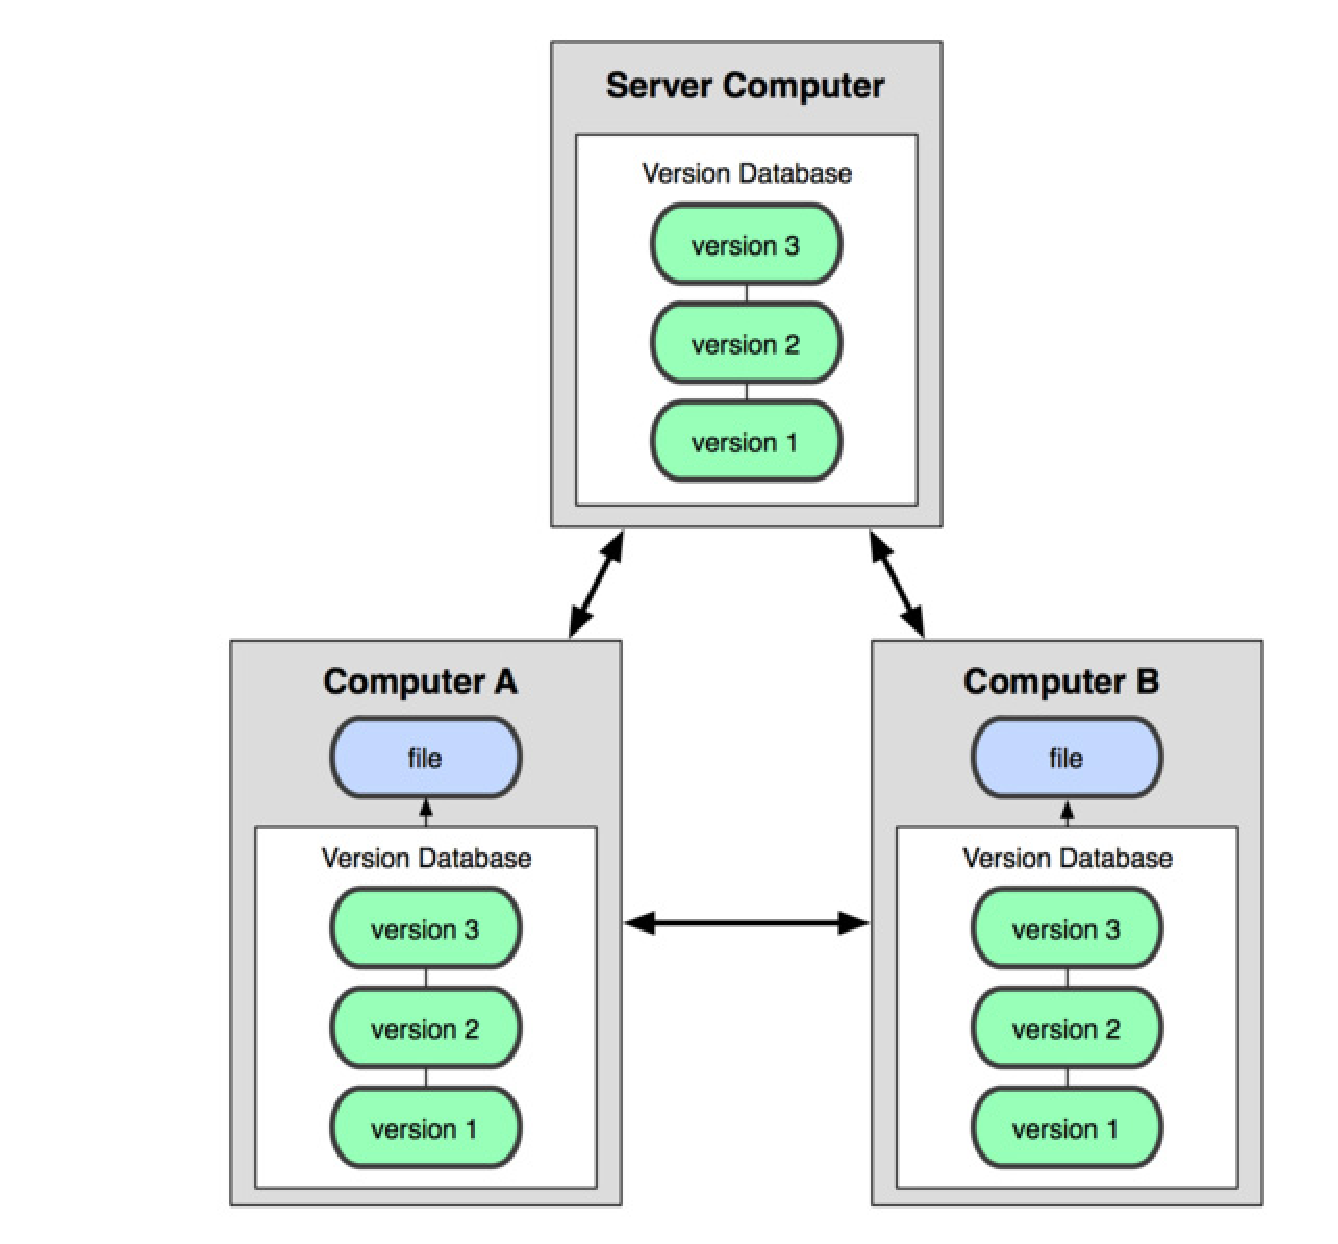
\includegraphics[width=300px]{./eps/git/git_diag_cv_distribuido.eps}
  \caption{Diagrama de control de versiones distribuido}
  \label{fig:cvdistrib}
\end{figure}

\subsection{Acerca de Git}

Debido al fuerte apoyo de la comunidad y su gran uso comercial, se selecciona como herramienta para la gestión de versiones. Así mismo, se han analizado sus ventajas frente a SVN (capítulo \ref{sec:git_vs_svn} en apéndice \fullref{ap:git})

Git (referencia en apéndice \fullref{ap:git}) es un software de control de versiones diseñado por Linus Torvalds, pensando en la eficiencia y la confiabilidad del mantenimiento de versiones de aplicaciones cuando estas tienen un gran número archivos de código fuente. Al principio, Git se pensó como un motor de bajo nivel sobre el cual otros pudieran escribir la interfaz de usuario o front-end. Sin embargo, Git se ha convertido desde entonces en un sistema de control de versiones con funcionalidad plena. Hay algunos proyectos de mucha relevancia que ya usan Git, en particular, el grupo de programación del núcleo Linux.

El flujo de trabajo básico en Git es:
\begin{enumerate}
	\item{Modificar una serie de archivos en directorio de trabajo.}
	\item{Preparar los archivos, añadiendo instantáneas de ellos al área de preparación.}
	\item{Confirmar los cambios, lo que toma los archivos tal y como están en el área de preparación, y almacena esa instantánea de manera permanente en el directorio de Git remoto.}
\end{enumerate}
	

% Características de Git
\subsubsection {Características}

El diseño de Git se basó en BitKeeper \footnote{BitKeeper es el sistema de gestion de codigo fuente usado en inicios para el kernel de Linux. BitMover (el fabricante) decidió no mantener la versión gratuita por motivos de rentabilidad económica.} y en Monotone. 
Sus principales características son:

\begin{itemize}
	\item{
		Fuerte apoyo al desarrollo no-lineal, por ende rapidez en la gestión de ramificaciones y mezclado de diferentes versiones. Git incluye herramientas específicas para navegar y visualizar un historial de desarrollo no-lineal. Una presunción medular en Git es que un cambio será fusionado mucho más frecuentemente de lo que se escribe originalmente, conforme se pasa entre varios programadores que lo revisan.
	}
	\item{
		Gestión distribuida. Git le da a cada programador una copia local del historial del desarrollo entero, y los cambios se propagan entre los repositorios locales. Los cambios se importan como ramificaciones adicionales y pueden ser fusionados en la misma manera que se hace con la ramificación local.
	}
	\item{
		Los almacenes de información pueden publicarse por HTTP, FTP, rsync o mediante un protocolo nativo, ya sea a través de una conexión TCP/IP simple o a través de cifrado SSH. Git también puede emular servidores CVS, lo que habilita el uso de clientes CVS pre-existentes y modulos IDE para CVS pre-existentes en el acceso de repositorios Git.
	}
	\item{
	 	Los repositorios Subversion y SVK se pueden usar directamente con git-svn.
	}
	\item{
		Gestión eficiente de proyectos grandes, dada la rapidez de gestión de diferencias entre archivos, entre otras mejoras de optimización de velocidad de ejecución.
	}
	\item{
		Todas las versiones previas a un cambio determinado, implican la notificación de un cambio posterior en cualquiera de ellas a ese cambio (denominado autenticación criptográfica de historial).
	}
\end{itemize}


% ----------------------------------
% Sec Textmate como editor de textos
% ----------------------------------
\section{Textmate como editor de textos} % (fold)
  \label{sec:textmate_como_editor_de_textos}
  
  Probablemente, la herramienta de software con la que pasemos más tiempo en nuestro trabajo diario como programadores sea el editor de código. Es por ello que la importancia de elegir un buen editor se convierte en primordial, y es probablemente una de las selecciones más cuidadosas que debemos hacer si queremos que nuestra productividad no sufra.

  Textmate es un editor de textos de pago con interfaz GUI para Mac OS X, creado por Allan Odgaard. La ventaja principal ante usar entornos de programación específicos es que es un editor altamente personalizable, que consume muy pocos recursos y que es capaz de soportar la compilación de diferentes lenguajes. Además, cuenta con ayudas de teclado (conocidas como «macros») para aumentar la productividad de programación. 

  No es un IDE, es decir, no pretende abarcar todas y cada una de las posibilidades que contemple tu plataforma de desarrollo. Pero lo cierto es que gracias a las extensiones en forma de {\it snippets} de código, macros, y otros, se puede convertir perfectamente en el centro de control absoluto durante el desarrollo de tu proyecto. Y todo esto siendo muchísimo más ligero que los tradicionales IDE, con la ventaja adicional de ser agnóstico (no todos los IDE lo son) en cuanto a las herramientas extra que estemos usando: compilador, sistema de control de versiones, etc.  

  Algunas de las características más destacadas de este editor son:
  
  \begin{itemize}
    \item Búsqueda y reemplazo de texto en un proyecto (ideal para refactorizaciones).
    \item Búsqueda y reemplazo de texto por expresiones regulares.
    \item Autoindentado en acciones comunes, como pegar texto.
    \item Autoemparejado de corchetes y otros caracteres.
    \item Histórico del portapapeles.
    \item Selector de texto por columnas y escritura en varias líneas a la vez en una misma columna (ideal para añadir un prefijo común a varias líneas de código, por ejemplo).
    \item Autocompletado de palabras de entre las que aparecen en el documento actual.
    \item Selectores para limitar el alcance de las acciones y las preferencias del editor.
    \item Bloques de código plegables.
    \item Grabación de macros (para crearlas sin necesidad de programarlas).
    \item Cambio rápido a cualquier fichero del proyecto tecleando parte de su nombre.
    \item Ejecutar comandos del sistema en el contexto de un documento.
    \item Navegación entre ficheros por pestañas.
    \item Soporte para más de 50 lenguajes.
    \item Soporte para casi todos los sistemas de control de versiones.
    \item Personalización del editor a través de temas.
  \end{itemize}

  % ----------------------------------
  % Sub Snippets
  % ----------------------------------
  \subsection{Snippets} % (fold)
    \label{sub:textmate_snippets}
  
    Los {\it snippets} permiten insertar porciones de código en el fichero que se esté editando de forma muy sencilla y moverse rápidamente por el texto personalizable de dicho {\it snippet}. Se pueden contextualizar, de modo que ciertos {\it snippets} sólo se puedan utilizar si se está editando un determinado tipo de fichero.

    Los {\it snippets} son accesibles desde la opción de menú {\it Bundles}, donde están ordenados por contexto (habitualmente, el lenguaje o entorno de programación que se esté usando). Aunque lo mejor es lanzarlos creando para ellos una secuencia de caracteres, tras las que, al pulsar tabulador, se ejecuta.

  % subsection snippets (end)
  
  % ----------------------------------
  % Sub Comandos
  % ----------------------------------
  \subsection{Comandos} % (fold)
    \label{sub:textmate_comandos}
    
    Los comandos en TextMate permiten ejecutar un código arbitrario (definido por una extensión en particular), el cual puede estar escrito en un lenguaje de programación. TextMate define una serie de variables de entorno con información como la línea actual, la ruta al proyecto, el fichero que se está editando, el texto seleccionado, etc. El comando sólo tiene que tomar la información que necesite y actuar en consecuencia. El resultado de ejecutar dicho comando puede introducirse directamente en el punto donde estaba situado el cursor, reemplazar todo o parte del texto, crear un nuevo documento y pegarse en él, etc.

    Los comandos son accesibles también desde el menú {\it Bundles}, o se pueden asignar a la pulsación de ciertas teclas para que se lancen. Su activación puede depender de que estés en el contexto adecuado, de modo que puedes usar la misma combinación de teclas para distintos comportamientos según estés editando código en Ruby, en C o en Java. 
    
  % subsection comandos (end)

% section textmate_como_editor_de_textos (end)

% ----------------------------------
% Sec PivotalTracker como gestor de proyectos ágiles
% ----------------------------------
\section{Pivotal Tracker como gestor de proyectos ágiles} % (fold)
  \label{sec:pivotaltracker_como_gestor_de_proyectos_agiles}

  Es una herramienta gratuita de {\bf Pivotal Labs}. Está destinada a la gestión de proyectos ágiles, permitiendo organizar las tareas utilizando el concepto de gestión de pilas.
  
  La herramienta es recomendable para los desarrolladores y coordinadores de proyectos, así como para los clientes y agentes externos. La curva de aprendizaje es muy sencilla, lo cuál permite tomar esta herramienta en cualquier momento y probarla sin tener un costo adicional en cuanto a pérdida de tiempo.

  Cuenta con diversas fuentes de información y métricas para controlar, de una forma detallada, el progreso diario, semanal y mensual de un proyecto o de sus miembros.
  
  % ----------------------------------
  % Sub Familiarización con el entorno
  % ----------------------------------
  \subsection{Familiarización con el entorno} % (fold)
    \label{sub:familiarizacion_con_el_entorno}
    
    En las sucesivas secciones se detallará el uso de la aplicación para la gestión de los proyectos, así como se introducirá al lector para que pueda familiarizarse con la misma.
    
    % ----------------------------------
    % SubSub Pilas
    % ----------------------------------
    \subsubsection{Pilas} % (fold)
    \label{ssub:pilas}
      Las historias de usuario, que se asemejan a las tareas de cada uno de los requisitos que se desarrollará, se ordenan en distintas columnas denominadas {\bf pilas}. Hay 4 tipos de pilas:
      \begin{itemize}
        \item {\bf Current}. Historias de usuario planificadas para la iteración en la que estamos.
        \item {\bf Backlog}. Historias de usuario planificadas para iteraciones futuras. {\it Pivotal Tracker} define donde empiezan las iteraciones según la velocidad establecida. Con esto se puede conseguir una estimación a largo plazo del proyecto.
        \item {\bf Icebox}. Historias de usuario que algún día quizás se realicen. Por defecto, cuando se crea una historia nueva, se coloca en esta pila.
        \item {\bf Done}. Normalmente no se muestra. Se muestras las iteraciones pasadas. 
      \end{itemize}
      
      \begin{figure}[H]
        \centering
          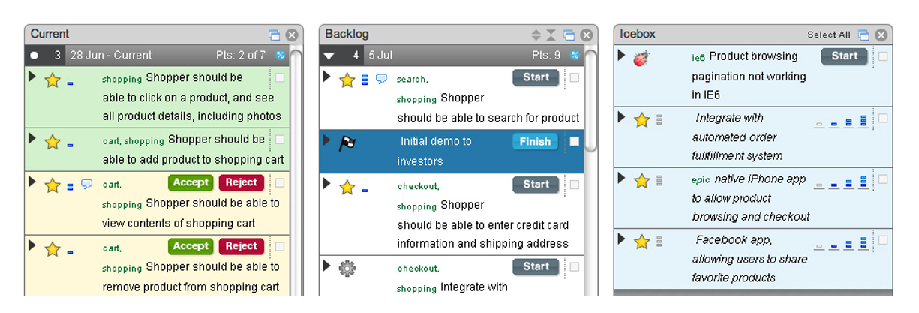
\includegraphics[width=15cm]{./eps/herramientas/pt/pt_pilas.eps}
        \caption{Tipos de pilas en Pivotal Tracker}
        \label{fig:pt_pilas}
      \end{figure}
      
    % subsubsection pilas (end)
  
    % ----------------------------------
    % SubSub Tipos de historias de usuario
    % ----------------------------------
    \subsubsection{Tipos de historias de usuario} % (fold)
    \label{ssub:tipos_de_historias_de_usuario}
      
      \begin{itemize}
        \item {\bf Feature}. Representadas por una estrella. Representan requisitos de usuario y las única que estiman (aportan valor de negocio al usuario). La velocidad se debería medir en funcionalidad de negocio capaz de realizar en una iteración).
        \item {\bf Bugs}. Modificaciones que hay realizar para mejorar un error.
        \item {\bf Chore} (trabajo rutinario). Representan tareas que hay que hacer y que no aportan valor de negocio ni son errores.
        \item {\bf Release}. Marcan hitos en el tiempo. Se tienen en cuenta en la planificación y en el cálculo de velocidad. Cuando se crea una release, se indica la fecha: si todo va bien saldrá en azul, pero si según la velocidad definida no dará tiempo a terminar todas las historias que hay por delante, se marcará en rojo.
      \end{itemize}
      
      \begin{figure}[H]
        \centering
          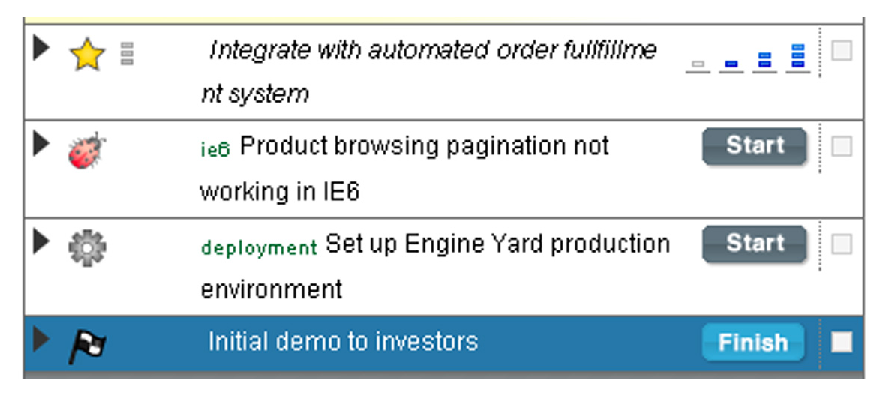
\includegraphics[width=11cm]{./eps/herramientas/pt/pt_historias.eps}
        \caption{Tipos de historias de usuario en Pivotal Tracker}
        \label{fig:pt_historias}
      \end{figure}
      
      Cada historia se puede modificar estableciendo el tipo, estimación de velocidad, etiquetas, estado, miembro, descripción, comentario y archivos adjuntos.
    % subsubsection tipos_de_historias_de_usuario (end)
    
    % ----------------------------------
    % SubSub Tipos de estados en historias
    % ----------------------------------
    \subsubsection{Tipos de estados en historias} % (fold)
    \label{ssub:tipos_de_estados_en_historias}
    
      Los estados vienen definidos por:
      \begin{itemize}
        \item {\bf Not Yet Started}. Todavía no se ha empezado a trabajar sobre la historia. Puede estar en cualquier pila menos {\it «done»}. 
        \item {\bf Started}. Se refiere a las historias comenzadas, es decir, en la que se está actualmente trabajando. Si dede cualquier pila se pulsa el botón de {\it «start»}, ésta pasa a la pila de {\it «current»}.
        \item {\bf Finished}. Estado para cuando se termina el desarrollo de la historia. Tras este punto, hay que pasar a otro que define la entrega al cliente.
        \item {\bf Delivered}. Historia entregada al cliente. Está a la espera de ser aceptada o denegada.
        \item {\bf Accepted}. El cliente acepta la historia como buena.
        \item {\bf Rejected}. El cliente deniega la historia. Se tiene que empezar a realizar de nuevo para volver a pasar la deliberación. 
      \end{itemize}
      
    % subsubsection tipos_de_estados_en_historias (end)
    
    % ----------------------------------
    % SubSub Planificación y cálculo de velocidad
    % ----------------------------------
    \subsubsection{Planificación y cálculo de velocidad} % (fold)
    \label{ssub:planificacion_y_calculo_de_velocidad}
      
      En principio la longitud de los sprints es de 1 semana. Se puede cambiar en las configuraciones del proyecto:  desde 1 semana hasta un máximo de 4.

      La estimación de las historias de usuario se hace en puntos de historia (recomendable). Por defecto tenemos los valores 0, 1, 2, 3, y son los cuadrados azules que se ven a la derecha de la historia de usuario.
      
      Si estos valores nos parecen insuficientes, los podemos cambiar en la configuración del proyecto. A elegir entre: potencias de 2 (0, 1, 2, 4, 8) o Fibonacci (0, 1, 2, 3, 5, 8).
      
      En función de la longitud de la iteración y de la velocidad media (cuantos puntos de historia hacemos en una iteración), Pivotal Tracker planificará las historias que somos capaces de hacer en las siguientes iteraciones. La velocidad se calcula, por defecto, como la media de las 3 últimas iteraciones; pero lo podemos configurar para que sea le media 1, 2, 3, o 4 iteraciones.
      
    % subsubsection planificación_y_cálculo_de_velocidad (end)
    
  % subsection familiarización_con_el_entorno (end)
  
  % ----------------------------------
  % Sub Aplicación a las metodologías ágiles
  % ----------------------------------
  \subsection{Aplicación a la Programación Extrema} % (fold)
    \label{sub:aplicacion_a_las_metodologias_agiles}
    
    La aplicación {\it Pivotal Tracker} está orientada a la metodología ágil, por lo que aplicarla a un método como la Programación Extrema (XP) no resulta difícil.

    Tal y como se estudió en secciones anteriores, los principios que una metodología ágil tiene son los siguientes:
      \begin{itemize}
        \item Individuos y sus interacciones más importantes que los procesos y las herramientas.
        \item Software que funciona es más importante que la documentación exhaustiva.
        \item La colaboración con el cliente en lugar de la negociación de contratos.
        \item La respuesta delante del cambio en lugar de seguir un plan cerrado.
      \end{itemize}

    Los últimos dos puntos están claramente cubiertos en Pivotal Tracker. En la fase de deliberación, cuando se aceptan o rechazan las historias finalizadas, el cliente (actuando como usuario) interactúa con el equipo de desarrollo. Así mismo, dado que las velocidades y estimaciones se pueden modificar, los cambios también pueden sostenerse.

    Las historias de usuario hay que definirlas de forma que los clientes puedan entenderlas, puesto que si orientan a los desarrolladores, los primeros pueden llegar a confundirse con la terminología.

    En XP, la planificación ha de realizarse por etapas, donde aparecerán diferentes iteraciones. En Pivotal Tracker, ésto se conoce como sprint o iteración. Se pueden definir como se ha visto anteriormente y establecer su duración (de 1 a 4 semanas). 

    En toda planificación hay que contemplar los errores. Pivotal Tracker define las historias de {\it bugs} para las que tienen que corregir errores. 

    Una iteración en XP supone una posterior versión pasando unos test de aceptación. Tras la aprobación del cliente se obtiene una pequeña entrega. En el diagrama de estados mostrado anteriormente, el proceso es similar.

    Para finalizar, la propiedad colectiva del código nos ayuda a definir el hecho de que en Pivotal Tracker, los programadores que formen parte del proyecto, deben escoger la primera de las historias mostradas en la pila de {\it «backlog»}. Éstos desarrollarán el código y posteriormente lo pasarán a revisión.
  
  % subsection aplicación_a_las_metodologías_ágiles (end)

% section pivotaltracker_como_gestor_de_proyectos_ágiles (end)

% ----------------------------------
% Sec Diigo como gestor de marcadores
% ----------------------------------
\section{Diigo como gestor de información} % (fold)
  \label{sec:diigo_como_gestor_de_informacion}

  Diigo es un sistema de gestión de información personal basado en el concepto «nube» \footnote{Computación en la nube o {\it Cloud computing}, es un paradigma que permite ofrecer servicios de computación a través de Internet.}, que incluye marcadores web, bloc de notas post-it, archivo de imágenes y documentos, así como selección de textos destacados.

  Diigo está disponible como un módulo insertado en el navegador para aumentar la productividad en el tratamiento y gestión de grandes cantidades de información. Se pueden resaltar párrafos interesantes y guardar como marcadores en la aplicación, con lo que la próxima vez que se acceda a esa información el usuario podrá focalizarse en lo que realmente le interesa.
  
  Lo que realmente hace a la herramienta interesante es su entorno colaborativo, a través del cuál varios integrantes de un mismo proyecto pueden compartir información usando etiquetas y enlaces. Se pueden crear grupos y hacer visible los marcadores a quien interese. Esto abre también la posibilidad de compartir con el resto de la comunidad de Diigo, con lo que los usuarios pueden suscribirse a temáticas para recibir enlaces sobre ella.  
  
% section diigo_como_gestor_de_información (end)


% ----------------------------------
% Sec Balsamiq Mockups para crear prototipos
% ----------------------------------
\section{Balsamiq Mockups para crear prototipos} % (fold)
  \label{sec:balsamiq_mockups_para_crear_prototipos}

  Balsamiq Mockups es una herramienta que nos permite realizar {\it wireframes} para webs fácilmente.

  Un {\it wireframe} (aplicado a la web) es una representación esquemática o prototipo de la solución que llevaremos adelante, sin entrar en etapas posteriores como el diseño gráfico o la programación web. Nos permite acordar con el cliente aspectos claves de la solución a desarrollar, como la distribución general de los elementos, sus jerarquías y la navegación de los mismos.

  Balsamiq Mockups nos provee de representaciones de todos los elementos utilizados para la construcción de una web: pantallas de navegadores, títulos, imágenes, videos, etc. Haciendo uso de ellos, sólo debemos organizarlos en un documento y ya podemos tener una primera aproximación de la solución a desarrollar. Dispone de más de 75 modelos ({\it stencils}) ya definidos con los diferentes elementos de las interfaces de usuario para montar prototipos.

  Esta es una herramienta que puede ser usada tanto por clientes como por desarrolladores.

  Los clientes pueden hacer uso de ello sin tener ningún tipo de conocimiento técnico especial. Gracias a ello, pueden comunicar de una manera más eficiente sus ideas y necesidades al grupo de trabajo que realiza los desarrollos técnicos.

  Los desarrolladores pueden usarlo con el mismo propósito, pero al revés. Para comunicar rápidamente las propuestas de solución, sin invertir demasiada cantidad de tiempo en esta primera etapa.

% section balsamiq_mockups_para_crear_prototipos (end)

%
% FIN DEL CAPÍTULO
%
\newpage
\thispagestyle{empty}